%!TEX root = ../main.tex
\chapter{Contexto experimental}
\label{chap:Contexto experimental}


En esta sección se expondrán los experimentos realizados basados en distintas fuentes de datos y distintas ontologías. La intención de este capítulo es demostrar que gracias a la utilización de ontologías es posible la interoperabilidad semántica y sintáctica entre distintas fuentes de datos. Para esto mostramos como realizar consultas al Punto SPARQL y pretendemos dar una pequeña demostración de casos prácticos utilizando fuentes de datos y ontologías reales ya existentes. 

Luego del despliegue del Punto SPARQL se procedió a organizar los experimentos. Para ello se definió el siguiente procedimiento:

Clasificar las consultas en casos específicos según complejidad sintáctica, semántica o computacional que se requiere teniendo también en cuenta el conjunto de fuentes de datos y ontologías utilizados para realizar las consultas correspondientes.
En cada caso se definieron consultas lo suficientemente claras y concisas que demuestren el funcionamiento correcto de la ontología utilizada para esa fuente de datos.

\begin{itemize}
    \item En el \textbf{caso 1} mostramos las bondades de trabajar con triplas RDF y ontologías.
    \item  En el \textbf{caso 2} consiste en mostrar la integración e interoperabilidad de dos fuentes y la facilidad de realizar consultas a modo de enriquecer la información obtenida.
    \item En el \textbf{caso 3} se pretende mostrar la integración e interoperabilidad con una ontología de dominio y una ontología general, para esto se utilizaron los datos de Procesos Licitatorios de la DNCP y también los datos disponibles en Wikidata.
    \item En el \textbf{Caso 4} se pretende mostrar la capacidad de reutilización e inferencia para la integración de datos utilizando la fuente de Procesos Licitatorios de la DNCP y la fuente de Procesos Licitatorios de Zaragoza, donde ambos reutilizan la ontología de Public Contract dentro de sus respectivas ontologías.
    \item Por último, en el \textbf{caso 5} se mejora la expresividad semántica de la ontología a fin de asegurar la correcta interpretación de los datos y facilita la consulta de los mismos.
\end{itemize}
  

En SPARQL es necesario definir primeramente todos los prefijos de las ontologías a utilizar en una determinada consulta. Los prefijos se definen de manera a facilitar la lectura de las consultas. De manera a facilitar la lectura de este documento las agrupamos en el Cuadro \ref{lst:prefijos}, los prefijos deben ir declarados antes de las consultas a realizar y solamente las ontologías utilizadas en esa consulta en específico.



\noindent\begin{minipage}[t]{\textwidth}
\begin{lstlisting}[captionpos=b, caption={Prefijos de las consultas SPARQL}, label={lst:prefijos},  numbers=left,  numberstyle=\tiny\color{mygray},frame=single]
    PREFIX foaf: <http://xmlns.com/foaf/0.1/>
    PREFIX co: <http://rhizomik.net/ontologies/copyrightonto.owl#>
    PREFIX oc: <http://opencoinage.org/rdf/>
    PREFIX ocd: <http://dati.camera.it/ocd/>
    PREFIX rdf: <http://www.w3.org/1999/02/22-rdf-syntax-ns#>
    PREFIX owl: <http://www.w3.org/2002/07/owl#>
    PREFIX lic: <http://example.org/licitaciones>
    PREFIX prov: <http://example.org/proveedores>
    PREFIX ocds: <http://purl.org/onto-ocds/ocds#>
    PREFIX dncp: <http://purl.org/onto-ocds/ocds/dncp.owl#>
    PREFIX pc: <http://purl.org/procurement/public-contracts#>
    PREFIX xsd:   <http://www.w3.org/2001/XMLSchema#>
    PREFIX fd: <http://foodable.co/ns/>
    PREFIX wd: <http://www.wikidata.org/entity/>
    PREFIX wdt: <http://www.wikidata.org/prop/direct/>
    PREFIX wikibase: <http://wikiba.se/ontology#>
    PREFIX p: <http://www.wikidata.org/prop/>
    PREFIX ps: <http://www.wikidata.org/prop/statement/>
    PREFIX pq: <http://www.wikidata.org/prop/qualifier/>
    PREFIX rdfs: <http://www.w3.org/2000/01/rdf-schema#>
    PREFIX bd: <http://www.bigdata.com/rdf#>
    PREFIX dbpedia-owl: <http://dbpedia.org/ontology/>
    PREFIX pproc: <http://contsem.unizar.es/def/sector-publico/pproc#> 
    PREFIX dcterms: <http://purl.org/dc/terms/> 
    PREFIX pc: <http://purl.org/procurement/public-contracts#> 
    PREFIX s: <http://schema.org/> 
    
 \end{lstlisting}
\end{minipage}

 A continuación se explica en cada caso los datos utilizados y cual es la intención. También se muestra cuál fue la consulta realizada al Punto SPARQL.


\section{Caso 1. Consultas de una fuente de datos a una ontología}


Aquí se pretende dar una demostración de cómo realizar una consulta simple a una fuente de datos y una ontología. Para esto se utilizó la Ontología OCDS y los datos de la DNCP. La consulta consiste en obtener de la base de datos toda la información referente a un proceso licitatorio, específicamente el proceso cuyo identificacor es <http://www.contrataciones.gov.py/datos/api/v2/doc/release/302438-adquisicion-semillas-gdc-1>, ya que es un Proceso Licitatorio que contemple las fases de Planificación, Convocatoria, Adjudicacion y Contratacion.

En el Cuadro \ref{lst:caso1} se muestra la consulta realizada al Punto SPARQL.

\noindent\begin{minipage}[t]{\textwidth}
\begin{lstlisting}[captionpos=b, caption={Tripas referente al proceso licitatorio cuyo identificacor es 302438}, label={lst:caso1},  numbers=left,  numberstyle=\tiny\color{mygray},frame=single]
SELECT *  
where {    	
<http://www.cont...e/302438-adquisicion-semillas-gdc-1> rdf:type ocds:Release .
<http://www.cont...ase/302438-adquisicion-semillas-gdc-1> ?propiedadNivel1 ?recursoNivel1 .   
OPTIONAL { ?recursoNivel1 ?propiedadNivel2 ?recursoNivel2}
}  
 \end{lstlisting}
\end{minipage}

 Si se considera el resultado de esta consulta un árbol, donde la raíz es el Proceso Licitatorio, entonces la consulta traerá la información del proceso licitatorio hasta el segundo nivel del árbol.

En la Figura \ref{img:caso1Resultado} se muestran los resultados obtenidos. Los nodos de un nivel representan un recurso o un literal. Se puede observar que el resultado contiene tanto los datos propios del Proceso de Contratación (Release) como es “ocds:ReleaseTag” cuyo valor es “compiled” y también contiene datos del Comprador (ocds:buyer) del bien o servicio como puede ser el título (ocds:organizationName) cuyo valor es “Gobierno Departamental de Central”. El valor “compiled” fue posible obtener a partir de la sentencia de la línea 4 y el valor “Gobierno Departamental de Central” a partir de la sentencia de la línea 5.

En la línea 3 encontramos la restricción cuya intención es asegurar que el recurso se trate de un Release, esto es posible debido a la utilización de la ontología desarrollada. En la línea 4 se consulta por el conjunto de triplas que cumplan la condición de tener como sujeto la IRI del proceso licitatorio. Con dicha sentencia, se obtiene una serie de triplas correspondientes a todas las relaciones de dicho proceso. Con la sentencia de la línea 5 se obtienen las triplas que tengan como sujeto el objeto proveniente del resultado de la primera sentencia. En otras otras palabras, se obtienen datos provenientes del segundo nivel del árbol. Haciendo esta segunda sentencia opcional, se puede también desplegar aquellas triplas que no tienen un segundo nivel en el árbol, por ende se muestran los datos directos del Proceso Licitatorio.

Como podemos ver en el Cuadro \ref{lst:caso1} , no es necesario conocer las propiedades, tipos de datos ni relaciones existentes entre los conceptos para realizar la consulta, es decir nos permite realizar consultas donde el modelo de datos no es necesariamente conocido. El único dato necesario fue la URI de un Proceso de Contratación. En cambio, si comparamos con una consulta en una base de datos relacional, para obtener todos los datos de un Proceso de Contratación, posiblemente se requeriría realizar un JOIN entre varias tablas relacionadas. Para poder realizar esto necesitaríamos conocer cuáles son las tablas involucradas y cuáles son las columnas para aplicar el JOIN correctamente.



\begin{figure}[ht!]
    \centering
    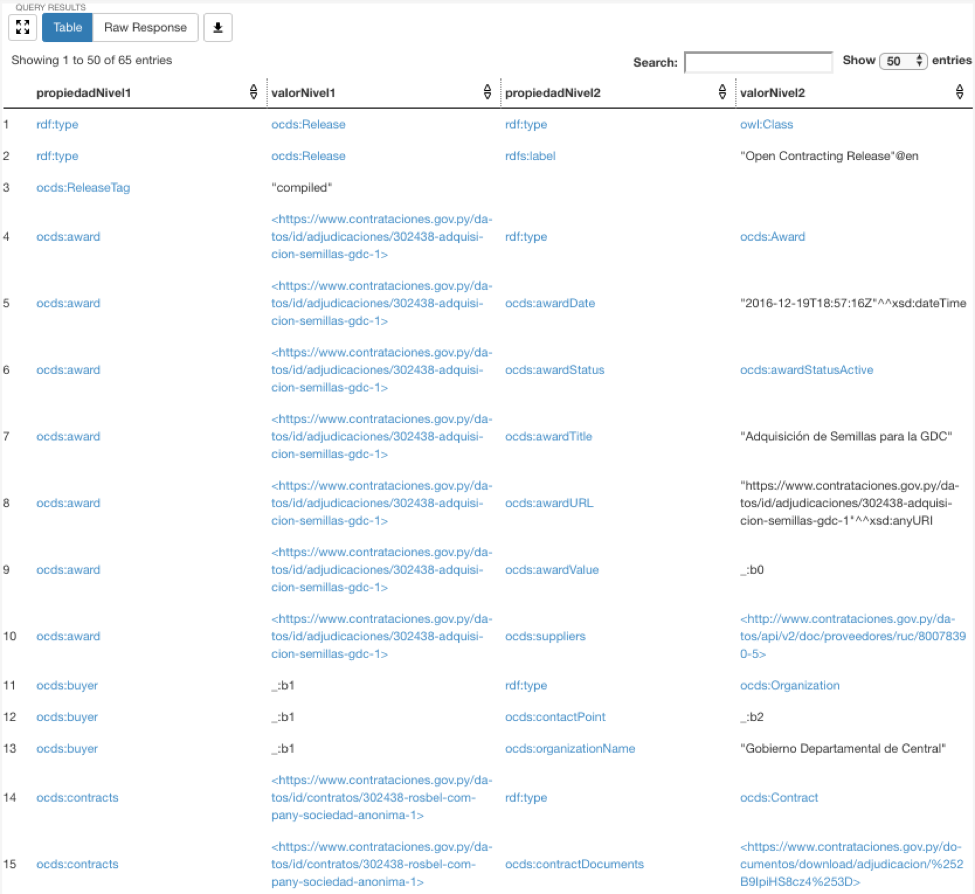
\includegraphics[width=150mm]{figuras/caso1Resultado.png}
    \caption{Despliegue de resultado de la consulta de l caso 1}
    \label{img:caso1Resultado}
 \end{figure}

\section{Caso 2. Dos fuentes de datos y dos ontología.}


Este caso consiste en la integración e interoperabilidad de dos fuentes con semántica enriquecida por el uso de dos ontologías. Se pretende demostrar la facilidad de realizar consultas a dos fuentes de datos a modo de enriquecer la información obtenida.

Se ejecutó una consulta al punto SPARQL que utiliza por un lado la ontología de OCDS y los datos de los procesos licitatorios de la DNCP y por otro lado la ontología desarrollada por la DNCP y los datos de Proveedores. En este caso el publicador de los datos es el mismo, pero las ontologías son distintas.

La consulta presentada en el cuadro \ref{lst:caso2} consiste en obtener datos de una organización cuyo RUC es 80008004-1. Se utiliza el comando SERVICE para realizar consultas a una fuente de datos distinta indicando su URL.

\noindent\begin{minipage}{\textwidth}
\begin{lstlisting}[captionpos=b, caption={Consulta a dos fuentes de de datos}, label={lst:caso2},  numbers=left,  numberstyle=\tiny\color{mygray},
    basicstyle=\tiny,frame=single]
SELECT  *
    WHERE
          {   
             { SELECT DISTINCT   ?c ?d
                WHERE
                  { ?organization
                              rdf:type          ocds:Organization ;
                              ocds:identifier    ?identifier .
                    ?identifier  ocds:identifierId  "80008004-1" .
                    ?organization
                              ?a                 ?b
                    OPTIONAL
                      { ?b  ?c  ?d }
                  }
              }
            UNION {
            SERVICE <http://localhost:3030/proveedores_completas_no_inf/sparql>
                  {  ?empresa  rdf:type  dncp:Proveedor ;
                          dncp:ruc   "80008004-1" ;
                          ?x         ?y
                  }
          }
          }
    
 \end{lstlisting}
\end{minipage}

 En la imagen \ref{img:caso2Resultado} se observan (a la izquierda) los datos obtenidos a partir de los Procesos Licitatorios utilizando la ontología OCDS y a la derecha se observan los datos obtenidos a partir de la fuente de datos de Proveedores que utiliza la ontología de la DNCP.


 \begin{figure}[ht!]
    \centering
    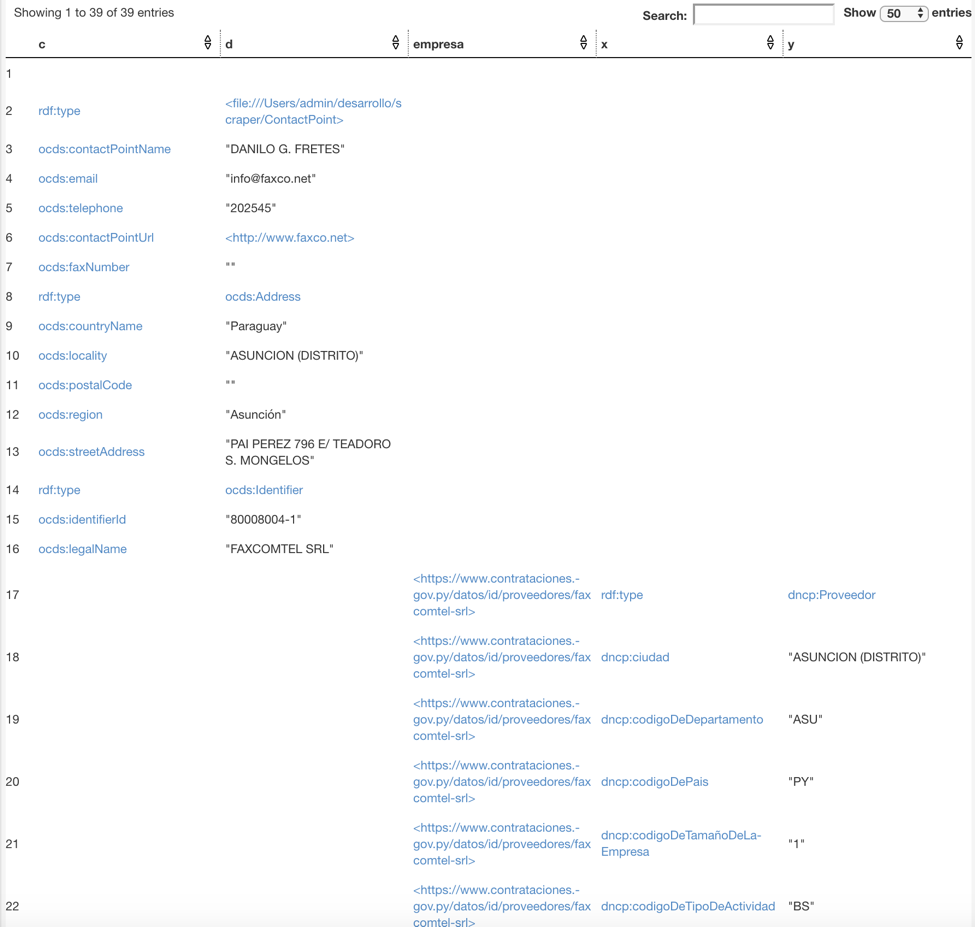
\includegraphics[width=150mm]{figuras/caso2Resultado.png}
    \caption{Despliegue de resultado de la consulta de l caso 2}
    \label{img:caso2Resultado}
 \end{figure}


 Se puede observar que ambas fuentes de datos pueden relacionarse entre sí a partir de la propiedad \textit{ocds:identifierId} y \textit{dncp:ruc.} Es posible realizar esta relación debido a que un experto de dominio puede deducir que ambas propiedades denotan los mismos valores. Esta igualdad entre propiedades no está explícitamente definida en la ontología. En el caso que se desee expresar de manera explícita esta información bastaría agregar la propiedad \textit{owl:equivalentProperty} a la definición de la propiedad \textit{identifierId}. Un ejemplo de cómo quedaría la definición de la propiedad \textit{identifierId} puede verse en el cuadro \ref{lst:caso2-2}. Con esto es posible utilizar indistintamente cualquiera de las dos propiedades para referirse a la misma relación.


 \begin{lstlisting}[captionpos=b, caption={Declaración de equivalencia semántica entre dncp:ruc y ocds:identifierID}, label=lst:caso2-2,  numbers=left,  numberstyle=\tiny\color{mygray},
    basicstyle=\tiny,frame=single]
###  http://purl.org/onto-ocds/ocds#identifierId
:identifierId rdf:type owl:DatatypeProperty ,
                        owl:FunctionalProperty ;
                owl:equivalentProperty dncp:ruc ;
                rdfs:domain :Identifier ;
                rdfs:range xsd:integer ,
                            xsd:string ;
                rdfs:comment "The identifier of the organization in the selected scheme."@en ;
                rdfs:label "Identifier ID"@en .
 \end{lstlisting}


 Las propiedades equivalentes tienen los mismos valores, pero pueden ser semánticamente diferentes, en este caso \textit{dncp:ruc} y \textit{ocds:identifierId} tienen el mismo valor, y \textit{dncp:ruc} se refiere al “Código Único del Contribuyente (RUC) de la Secretaría de Estado y Tributación (SET)” y \textit{ocds:identifierID} se refiere al “Identificador Único de la Organización”. En la tabla \ref{table:semanticaID} se expresa la comparación entre las propiedades mencionadas.

 Que dos individuos tengan una propiedad con el mismo valor no necesariamente implica que se trate del mismo individuo. En ontologías, a menos que haya una sentencia que indique que dos individuos son iguales o diferentes, no se puede asumir ninguna de las dos situaciones. 

 Como en los datos no está definida la equivalencia entre ambas instancias, entonces los datos obtenidos de las distintas fuentes deben ser asumidos como iguales por el conocimiento del experto de dominio. La forma de expresar explícitamente la igualdad semántica entre dos instancias seria agregando la sentencia de cuadro \ref{lst:caso2-1}. En la figura \ref{img:DiagramaCaso3} se observa como quedaría esta unión semántica entre ambas instancias.
 


 \begin{table}[!htbp]
    \centering
    \caption{Definición Semántica de Indentificador y RUC}
    \label{table:semanticaID}
    \resizebox{15cm}{!} {
    \begin{tabular}{|c|l|l|}
    \hline
    
Propiedad & Valor &  Significado \\ \hline

ocds:identifierID  & 80008004-1 &  Identificador de la Organización \\ \hline
Propiedaddncp:ruc & 80008004-1 &  Código Único del Contribuyente de la Secretaría de Estado y Tributación \\ \hline

    \end{tabular}
    }
    \end{table}



    \begin{lstlisting}[captionpos=b, caption=Declaracion de igualdad semantica de dos instancias, label=lst:caso2-1,  numbers=left,  numberstyle=\tiny\color{mygray},
        basicstyle=\tiny,frame=single]
<http://www.contrataciones.gov.py/datos/api/v2/doc/proveedores/ruc/80008004-1> 
owl:sameAs <http://www.contrataciones.gov.py/datos/id/proveedores/fax-comtel-srl>  .

     \end{lstlisting}

     \begin{figure}[ht!]
        \centering
        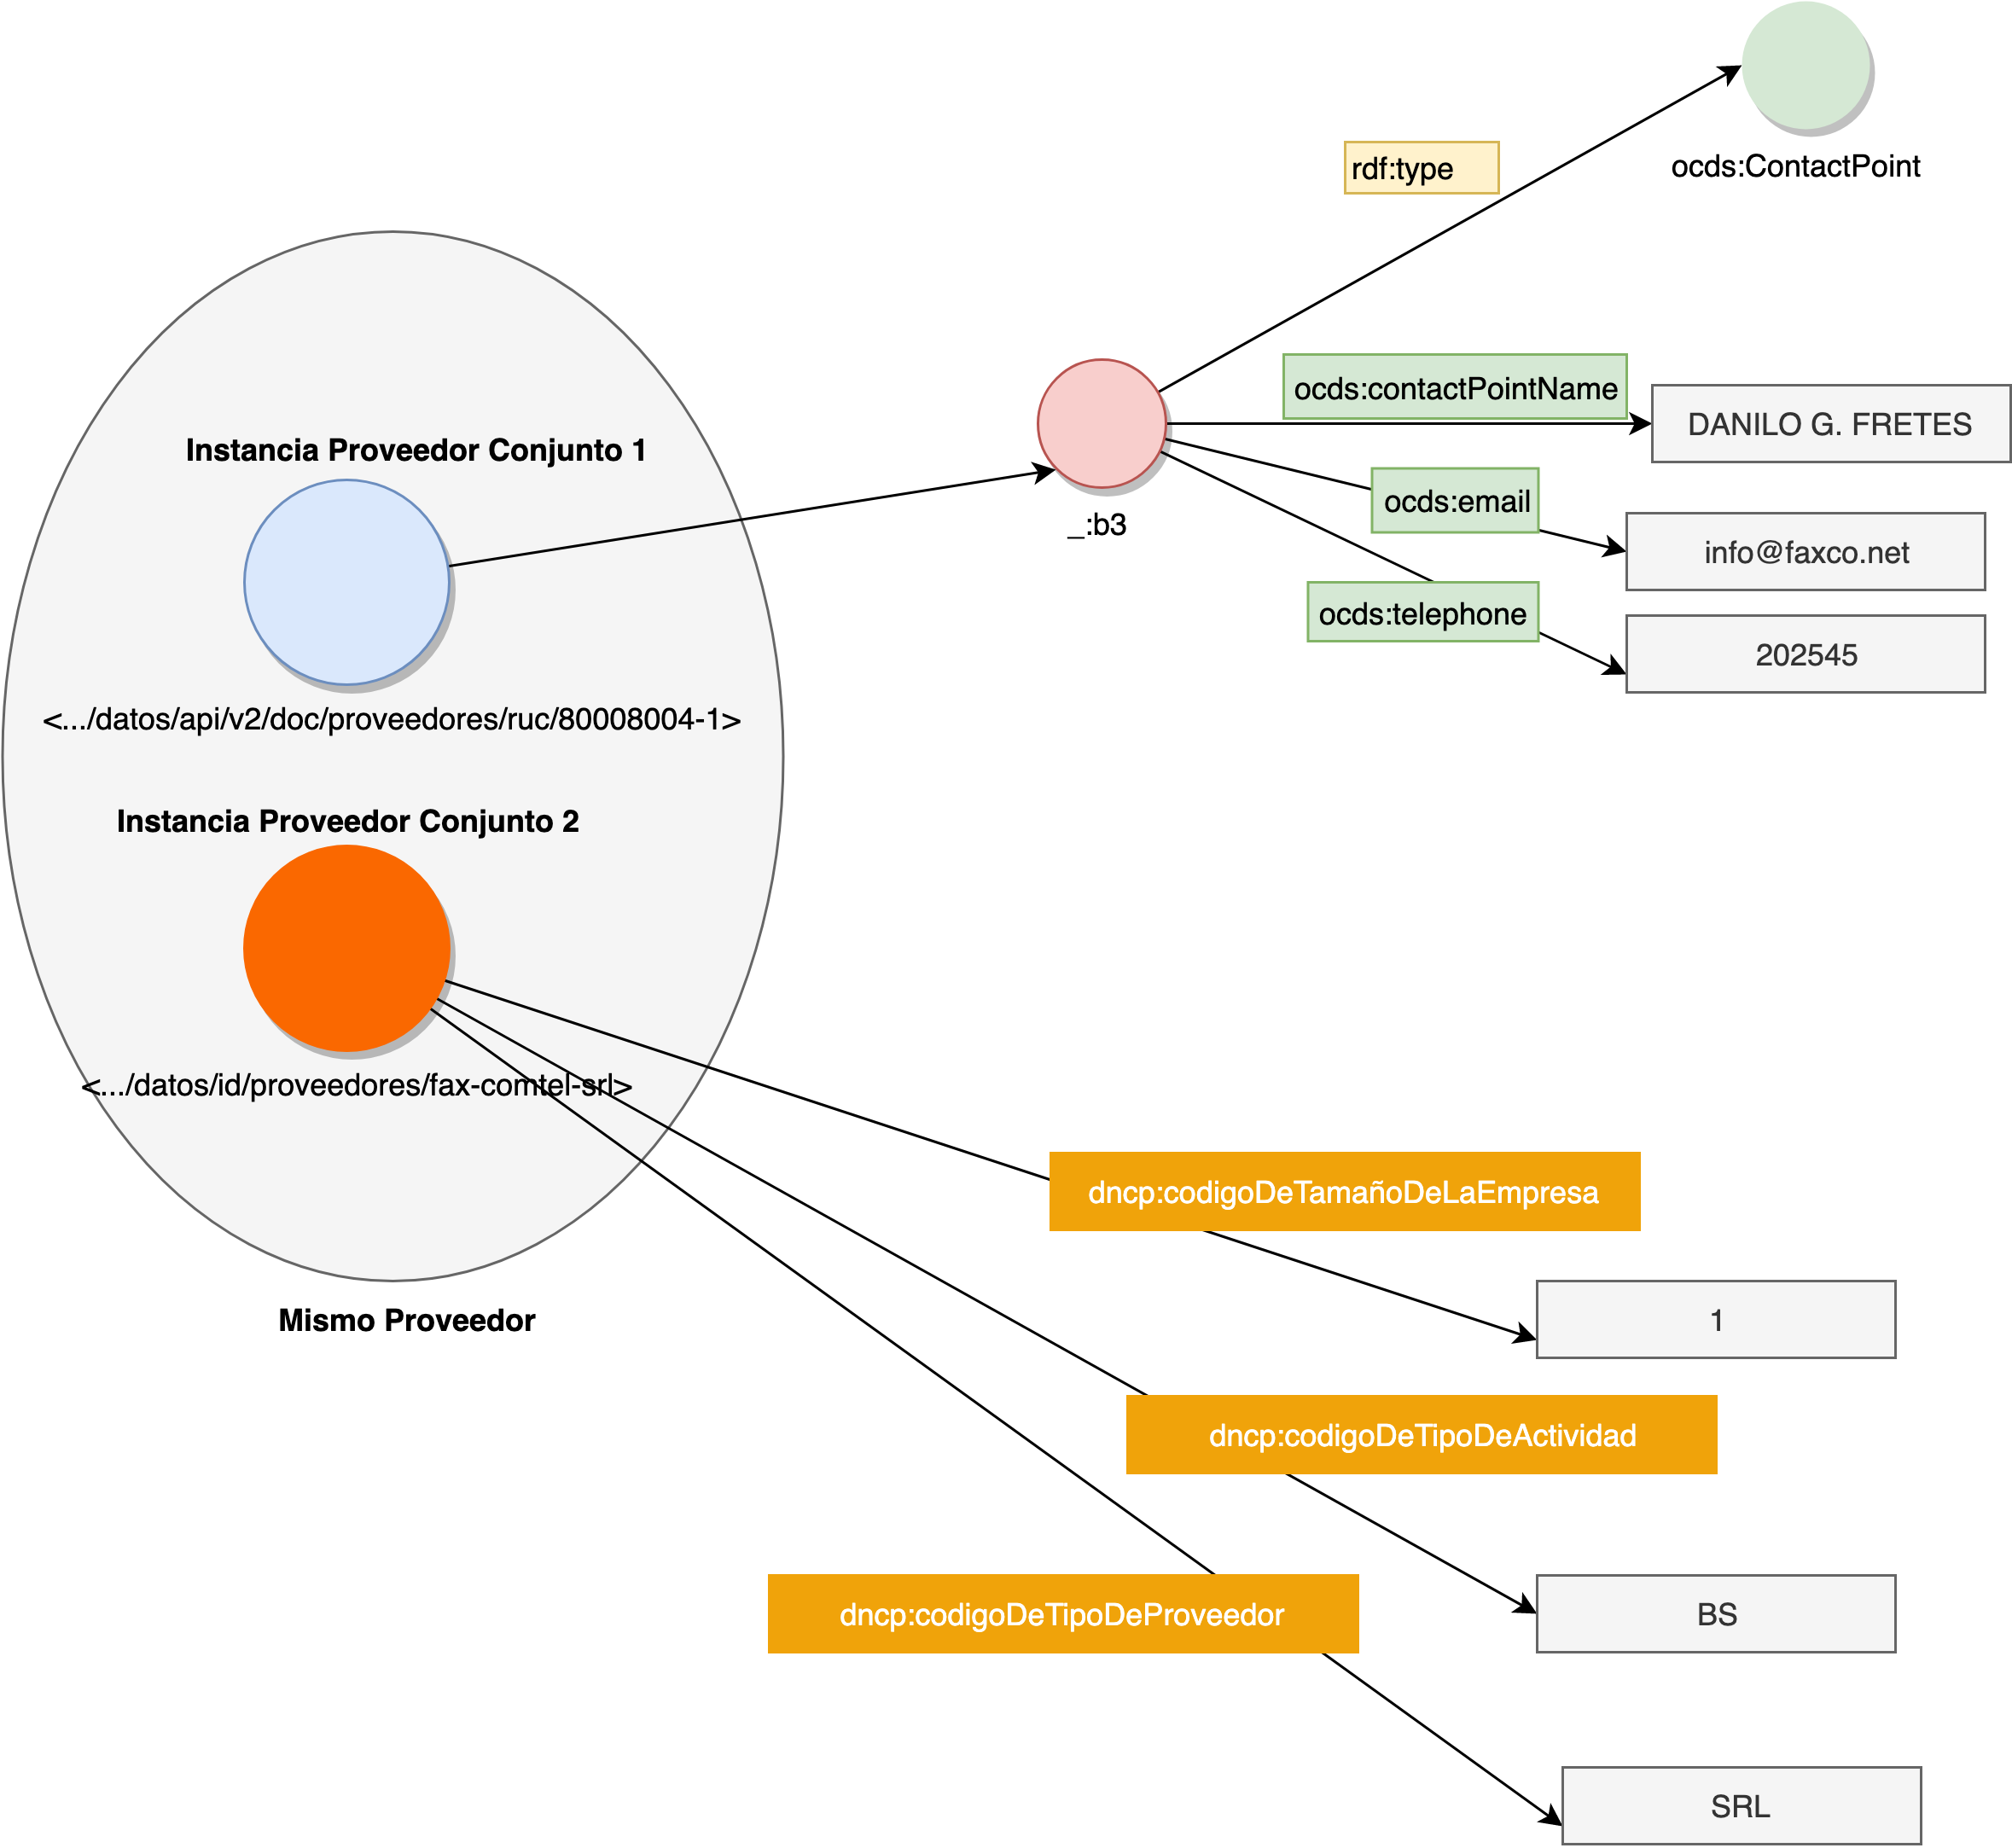
\includegraphics[width=150mm]{figuras/Diagramas-Caso2.png}
        \caption{Grafo de la consulta del caso 2}
        \label{img:DiagramaCaso2}
     \end{figure}

     Aquí se observa que ambos conjuntos de datos pertenecen al mismo Proveedor/Publicador y los datos de las organizaciones se complementan en cuanto a información se refiere. Por una parte podemos obtener datos como el nombre del punto de contacto (\textit{ocds:contactPointName}), email y teléfono. Por otra parte se pueden obtener datos como el código de tipo de proveedor, el cual en este ejemplo es “SRL”. 

    
\section{Caso 3. Dos fuentes de datos donde una es externa y dos ontologías}
\label{section:caso3}
Se pretende demostrar la integración e interoperabilidad con una ontología de dominio y una ontología general. Para esto, se utilizaron los datos de Procesos Licitatorios de la DNCP junto con la ontología OCDSPY, y también los datos disponibles en Wikidata\footnote{https://query.wikidata.org/} junto con su ontología propia. Con esto se enriqueció la fuente de datos primaria a partir de una fuente de datos externa, la cual permitió obtener más información relevante y contextual.

La consulta realizada en el Cuadro  \ref{lst:caso3-1} consiste en obtener la cantidad de todos los Procesos Licitatorios cuyos proveedores residen en países que no son limítrofes con Paraguay, agrupando estas cantidades de acuerdo al país.

\noindent\begin{minipage}[c]{\textwidth}
\begin{lstlisting}[captionpos=b, caption=Integración con una fuente de datos externa utilizando dos ontologías, label=lst:caso3-1,  numbers=left, numberstyle=\tiny\color{mygray},frame=single]
SELECT *
    WHERE {
        {
            SELECT ?label (COUNT(?label) AS ?cantidad)
            WHERE {
            ?plicitatorio rdf:type ocds:Release;
                          ocds:contracts ?contract.
            ?contract ocds:contractSuppliers ?org.
            ?org ocds:address ?b .
            ?b ocds:countryName ?label
                MINUS  { 
                    SERVICE <https://query.wikidata.org/sparql>{ 
                        SELECT DISTINCT  (str(?labelWhitLang) as ?label)
                            WHERE { 
                                    wd:Q733 wdt:P47 ?paislimitrofe .
                                    ?paislimitrofe wdt:P297 ?codigoPais.
                                    ?paislimitrofe rdfs:label ?labelWhitLang.
                                    FILTER (langMatches( lang(?labelWhitLang), "ES") )
                            }        
                    }
                }
            } GROUP BY ?label
        }
    }
 \end{lstlisting}
\end{minipage}

Primeramente se seleccionan todos los Procesos Licitatorios junto con el país donde residen (\textit{ocds:countryName}) excluyendo (MINUS) todos los países que sean limítrofes con Paraguay. En Wikidata, wd:Q733 es el identificador de país de Paraguay mientras que wdt:P47 es el identificador de la propiedad “comparte frontera con” y rdf:label es el nombre de país. El comando SERVICE nos permite realizar consultas a otro Punto SPARQL, en este caso Wikidata. La única información necesaria para lograr este enlace es conocer la URI que representa el Punto SPARQL para así poder realizar consultas sobre los datos externos.


Se utilizó el nombre del país en ambos conjuntos de datos como elemento de relación entre países para conseguir suprimir del resultado los países que son limítrofes con Paraguay. En la Figura \ref{img:caso3Resultado1} se muestran los resultados obtenidos.


\begin{figure}[ht!]
    \centering
    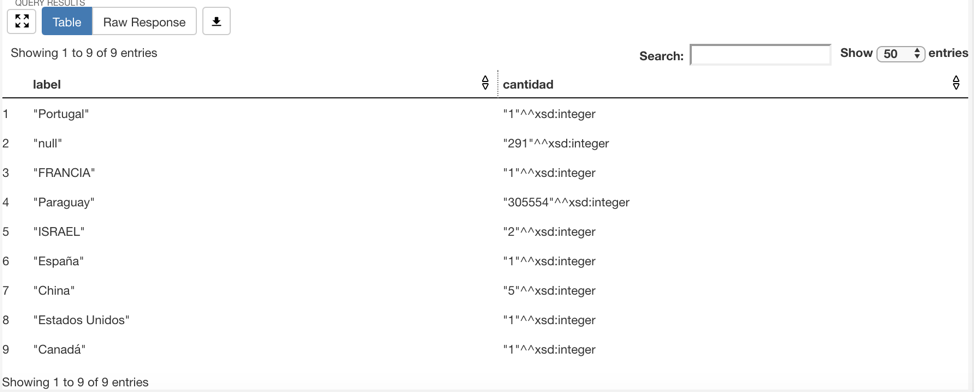
\includegraphics[width=150mm]{figuras/caso3Resultado1.png}
    \caption{Despliegue de resultado de la consulta del caso 3}
    \label{img:caso3Resultado1}
 \end{figure}


En la Figura \ref{img:caso3Resultado2} se ve el resultado si se suprime el filtro por países limítrofes correspondientes a las líneas desde la 11 a la 24. En la Figura \ref{img:DiagramaCaso3} se presenta un diagrama de relaciones entre las dos fuentes de datos, las ontologías utilizadas y la consulta.


 \begin{figure}[ht!]
    \centering
    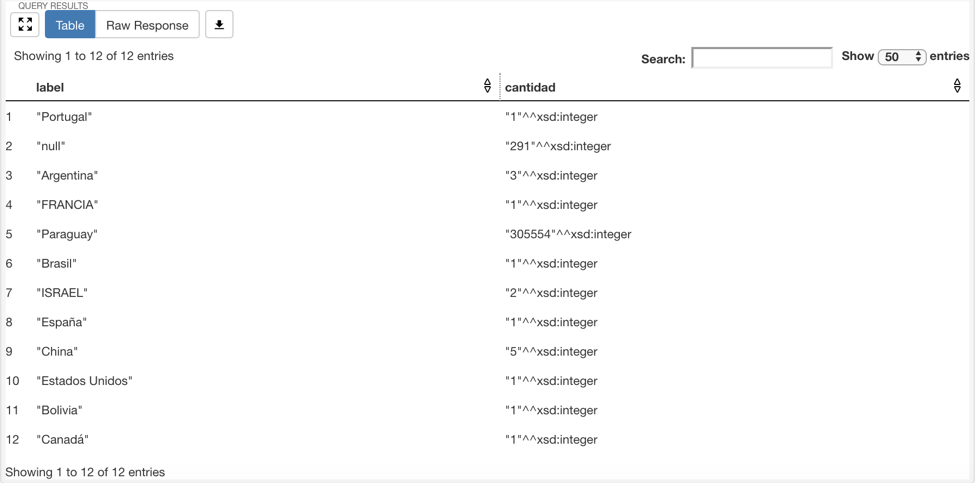
\includegraphics[width=150mm]{figuras/caso3Resultado2.png}
    \caption{Despliegue de resultado de la consulta del caso 3. Cantidad de todos los Procesos Licitatorios cuyos proveedores residen en países que no son limítrofes con Paraguay, agrupando estas cantidades de acuerdo al país}
    \label{img:caso3Resultado2}
 \end{figure}


 \begin{figure}[ht!]
    \centering
    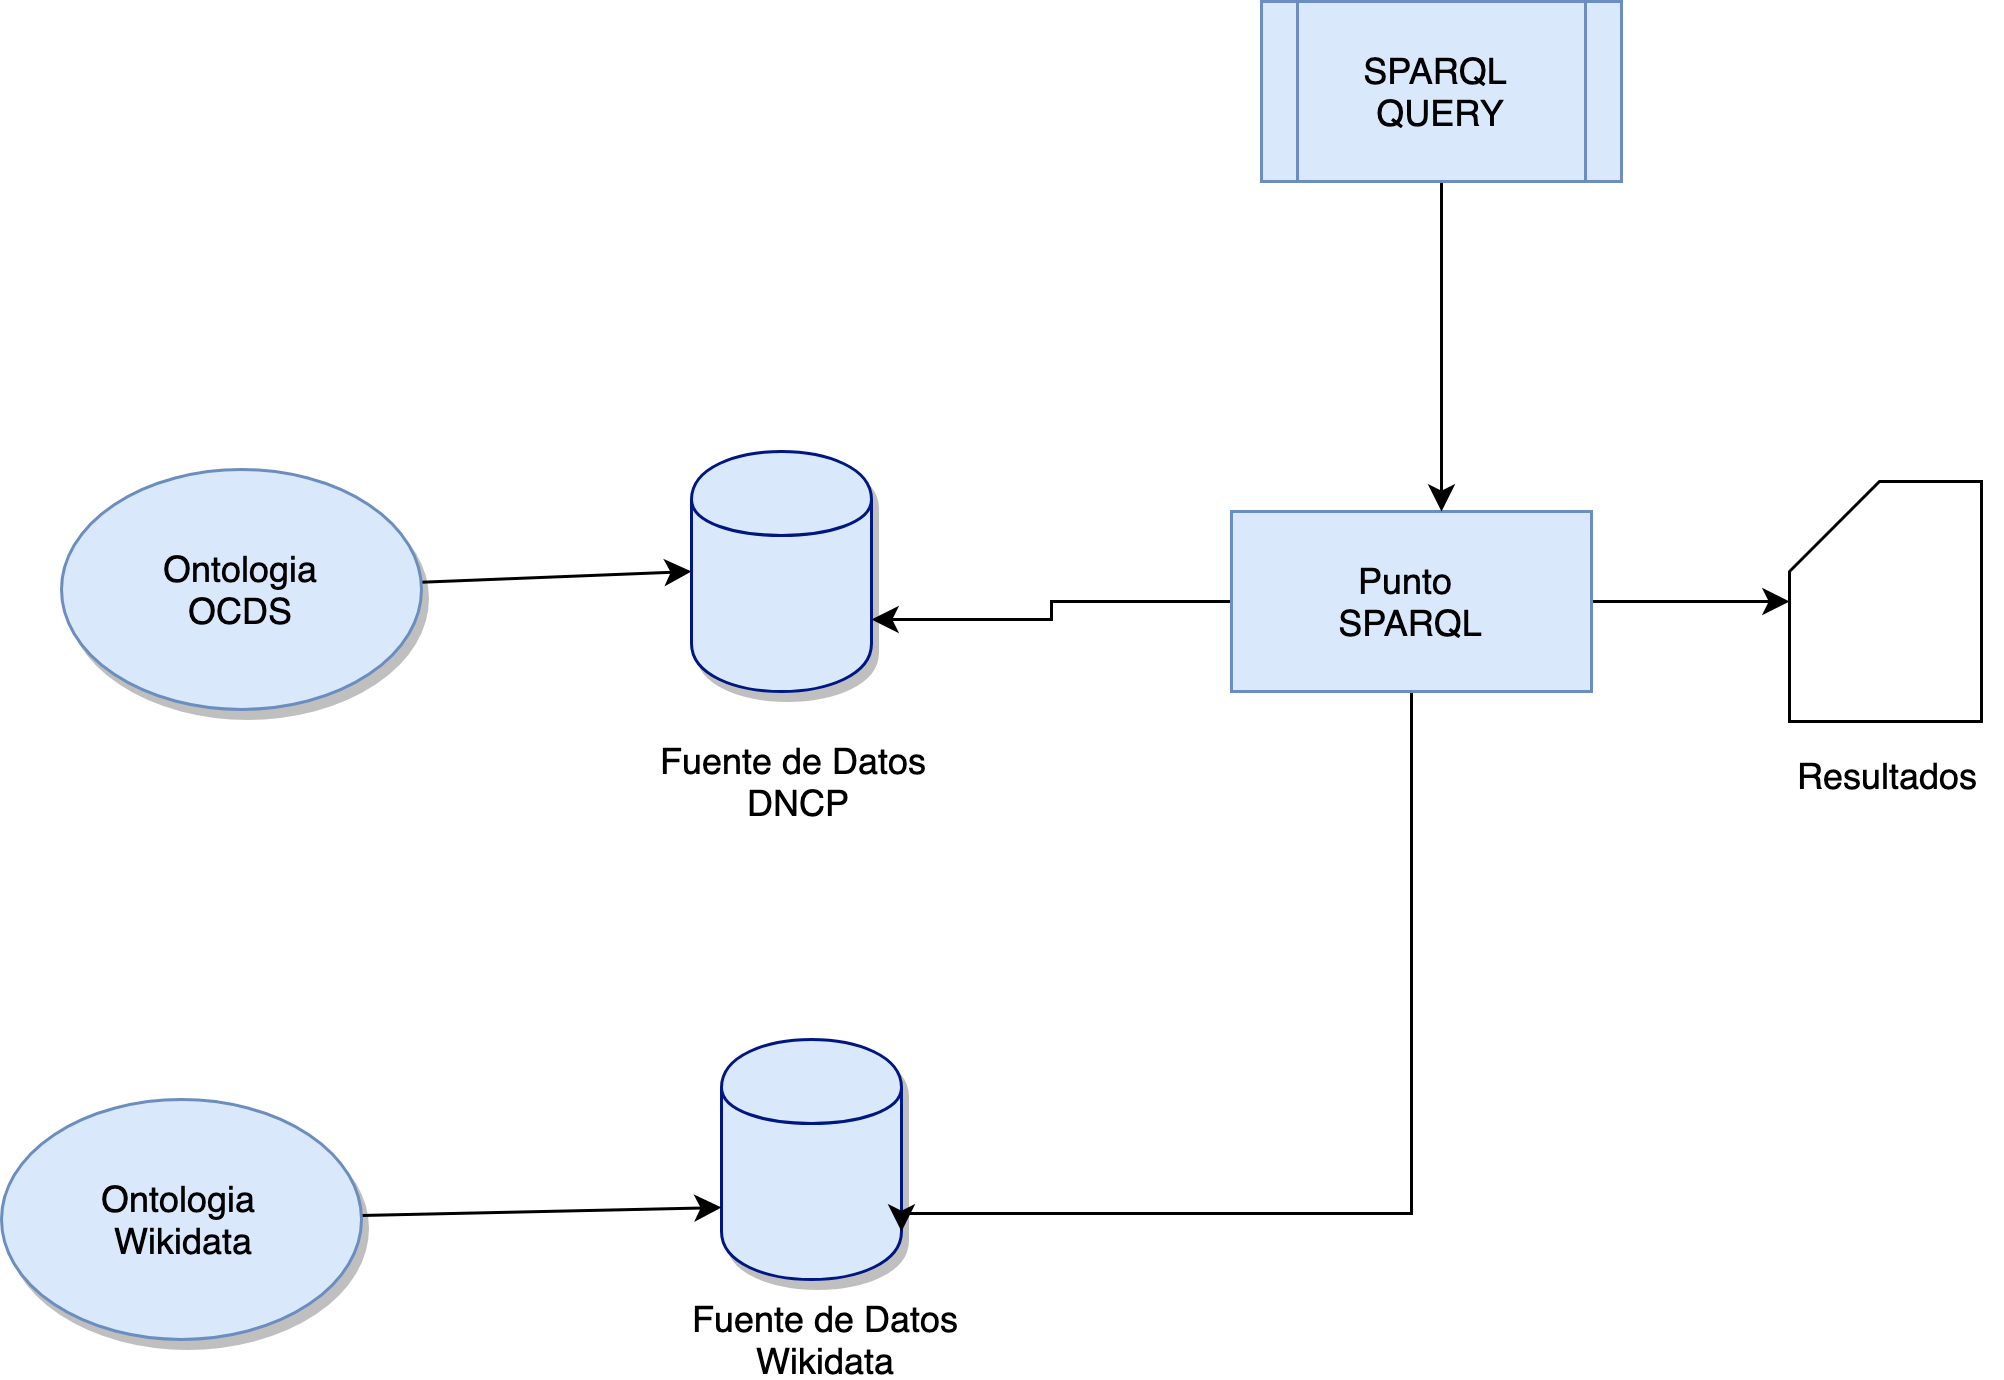
\includegraphics[width=150mm]{figuras/Diagramas-Caso3.png}
    \caption{Diagrama de la consulta del caso 3}
    \label{img:DiagramaCaso3}
 \end{figure}

Se tomó la decisión de utilizar este atributo debido a que no hay una relación directa entre un país en el conjunto de datos de la DNCP y el mismo país en el conjunto de datos de Wikidata, esto se podría mejorar con el técnica de la sección \ref{section:caso2mejora2}.

\subsection{Mejora: Transformación de literales a objetos}
Esta consulta podría tener inconvenientes si la forma de escribir del nombre de los país cambiara, es el caso de ISRAEL en la línea 5 de la Figura \ref{img:caso3Resultado1} que se encuentra en mayúsculas. Para evitar esto, lo óptimo sería que los atributos no sean de tipo texto sino más bien sean objetos dentro del conjunto de datos de la DNCP y éstos estén relacionados con otros semejantes dentro de la Web Semántica.

En el Cuadro \ref{lst:3-2} se muestra la definición actual de la propiedad “countryName” que pertenece a la clase “Address”. Se observa que el tipo de propiedad es “DatatypeProperty” el cual representa un literal.\hfill \break 

\noindent\begin{minipage}[c]{\textwidth}
\begin{lstlisting}[captionpos=b, caption=Definición de la propiedad countryName, label={lst:3-2},  numbers=left,  numberstyle=\tiny\color{mygray},frame=single]
###  http://purl.org/onto-ocds/ocds#countryName
:countryName rdf:type owl:DatatypeProperty ,
    owl:FunctionalProperty ;
    rdfs:domain :Address ;
    rdfs:range xsd:string ;
    rdfs:comment "The country name. For example, United States."@en ;
    rdfs:label "Country name"@en .
 \end{lstlisting}
\end{minipage}

 En el Cuadro \ref{lst:caso3-3} se muestra una solución al inconveniente mencionado. Primeramente se debe renombrar la propiedad \textit{countryName} a \textit{country} para que de esta forma denote la relación con un país y no con el nombre del país solamente. Luego se debe cambiar el rango de valores de \textit{rdfs: range xsd:string}  a \textit{rdfs:range :Country }donde \textit{Country} se refiere a una nueva clase a ser definida en la ontología. Esta última será la que represente al concepto “País”. Luego deberá definirse una instancia del país (por cada país que exista en la fuente de datos) de tipo \textit{Country}. Finalmente faltaría relacionar este recurso con otro semejante dentro de la Web Semántica, en este caso se puede realizar con los datos disponibles en Wikidata a través de la sentencia \textit{owl:sameAs wd:Q733} donde \textit{wd:Q733} es el identificador único (URI) de Paraguay en Wikidata.\hfill \break

\noindent\begin{minipage}[c]{\textwidth}
 \begin{lstlisting}[captionpos=b, caption=Declaración de la Clase Country, label={lst:caso3-3},  numbers=left,  numberstyle=\tiny\color{mygray},frame=single]
PREFIX wd: <http://www.wikidata.org/entity/>
###  http://purl.org/onto-ocds/ocds#country
:country rdf:type owl:ObjectProperty ,
                      owl:FunctionalProperty ;
             rdfs:domain :Address ;
             rdfs:range :Country ;
             rdfs:comment "El pais donde reside"@es ;
             rdfs:label "Pais de residencia"@en .

###  http://purl.org/onto-ocds/ocds#Country
:Country rdf:type owl:Class ;
         rdfs:comment "Representa un pais."@es ;
         rdfs:label "Pais"@es .

###  http://purl.org/onto-ocds/ocds#countryParaguay
:countryParaguay rdf:type owl:NamedIndividual ,
                                    :Country ;
                           dcterms:title "Republica del Paraguay"@es ;
                           rdfs:label "Paraguay"@es .
    owl:sameAs wd:Q733
 \end{lstlisting}
\end{minipage}

\section{Caso 4. Inferencia y Reutilización de ontologías. }

En este caso se pretende demostrar la capacidad de reutilización e inferencia para la integración de datos. Utilizamos la fuente de Procesos Licitatorios de la DNCP y la fuente de Procesos Licitatorios de Zaragoza, donde ambos reutilizan la ontología de Public Contract dentro de sus respectivas ontologías.

Para obtener las convocatorias de la DNCP es necesario que el Punto SPARQL utiliza el motor de inferencia ya que los datos no están anotados directamente con la propiedad \textit{pc:Tender} pero sí están anotados con \textit{ocds:Tender} la cual, en la ontología de OCDS, está definida como una subclase de \textit{pc:Tender} (como se muestra en el cuadro \ref{lst:caso4-1}). \hfill \break

\noindent\begin{minipage}[c]{\textwidth}
\begin{lstlisting}[captionpos=b, caption=Extension de la ontologia reutilizando PC, label={lst:caso4-1},  numbers=left,  numberstyle=\tiny\color{mygray},
    basicstyle=\footnotesize\ttfamily,frame=single]
###  http://purl.org/onto-ocds/ocds#Tender
:Tender rdf:type owl:Class ;
        rdfs:subClassOf pc:Tender ;
        rdfs:comment "Data regarding tender process - publicly inviting prospective contractors to submit bids for evaluation and selecting a winner or winners"@en ;
        rdfs:label "Tender"@en .
 \end{lstlisting}
\end{minipage}
 

 La consulta realizada en el cuadro  consiste en listar los primeros 6 contratos encontrados (3 de Paraguay y 3 de Zaragoza)”.
 
\noindent\begin{minipage}[c]{\textwidth}
 \begin{lstlisting}[captionpos=b, caption=Consulta a dos fuentes de datos utilizando el mismo concepto, label={lst:caso4-2},  numbers=left,  numberstyle=\tiny\color{mygray},
    basicstyle=\footnotesize\ttfamily,frame=single]
select ?tender
where {
    #Paraguay
    { select * 
    where 
    {?tender ?b pc:Tender } limit 3 
    }
    UNION 
    { 
    #Zaragoza
    SERVICE <http://datos.zaragoza.es/sparql> {
    SELECT * 
        WHERE {
        ?tender ?b pc:Tender 
        } limit 3
        }
    }
}
 \end{lstlisting}
\end{minipage}
 Los resultados obtenidos se muestran en la siguiente imagen \ref{img:caso4Resultado}. Allí se muestra el identificador de cada convocatoria. Con esta consulta, podemos estar seguros de que todos los recursos de la lista corresponden a convocatorias, aunque las convocatorias no son del mismo publicador de datos.



\begin{figure}[ht!]
    \centering
    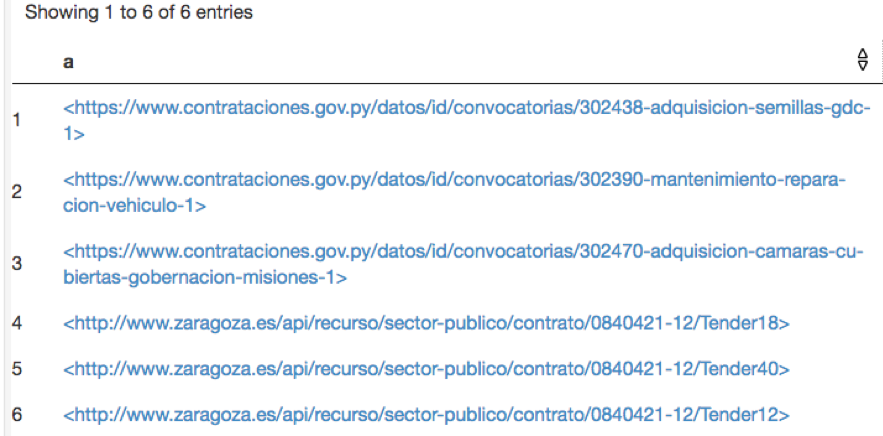
\includegraphics[width=150mm]{figuras/caso4Resultado.png}
    \caption{Despliegue de resultado de la consulta del caso 4}
    \label{img:caso4Resultado}
 \end{figure}


 En el gráfico \ref{img:Diagramas-Caso 4} se observa que ambas fuentes de datos reutilizan la ontología de Public Contract, en este caso la propiedad “Tender”. Gracias a esto es posible relacionar los datos en una consulta al Punto Sparql logrando así la interoperabilidad semántica, dando seguridad de que ambas fuentes de datos se refieren al mismo concepto.

 \begin{figure}[ht!]
    \centering
    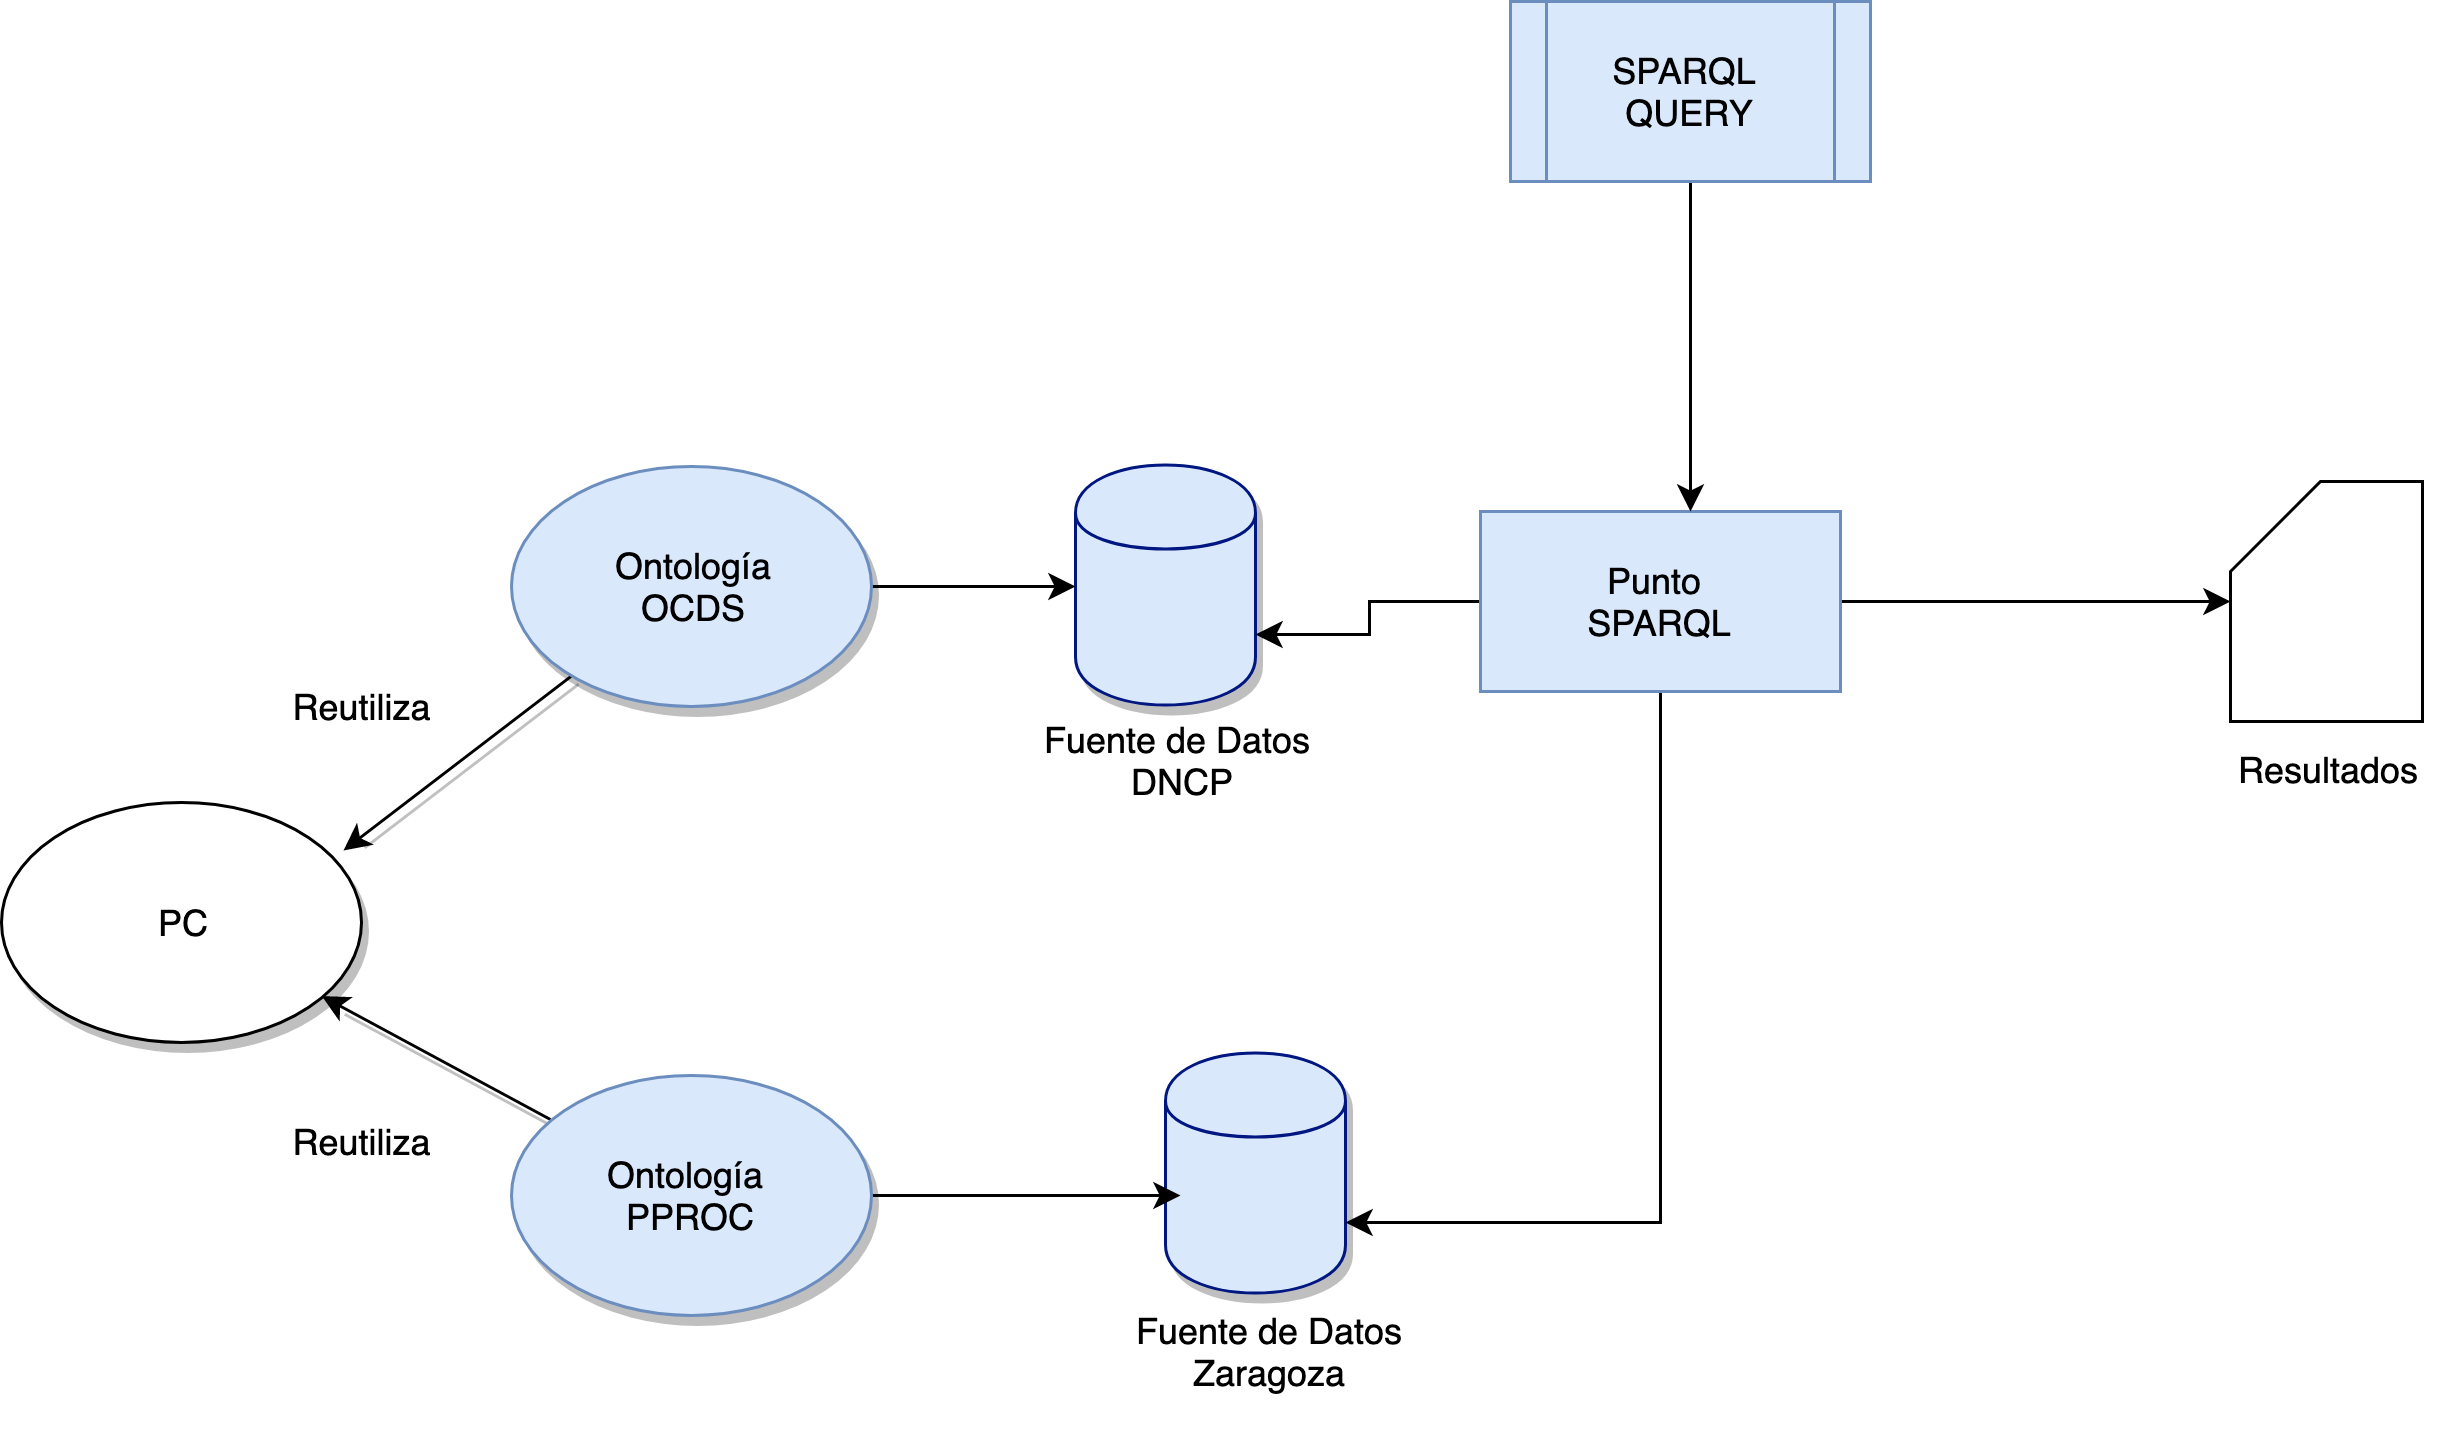
\includegraphics[width=150mm]{figuras/Diagramas-Caso4.png}
    \caption{Diagrama de la consulta del caso 4}
    \label{img:Diagramas-Caso 4}
 \end{figure}

\section{Caso 5. Mejora de la expresividad de la ontología. }

Se puede extender la capacidad semántica de la ontología actualizando el modelo ontológico sin que implique un alto costo debido a que éste se encuentra desacoplado de los datos.

Para este caso se utilizó la fuente de datos de procesos licitatorios y la ontología OCDS. Se define el concepto de “Proceso Licitatorio con Contrato” a través de una una clase (\textit{PLConContrato}) a partir de una restricción de propiedad. Esta clase se define como una subclase de \textit{Release}, que tiene como restricción todas las instancias de la clase \textit{Release} que tengan al menos una relación en la propiedad \textit{ocds:contracts}.


\begin{lstlisting}[captionpos=b, caption=Extension de la ontologia utilizando restricciones ontologicas, label={lst:caso5-1},  numbers=left,  numberstyle=\tiny\color{mygray},
    basicstyle=\small,frame=single]
INSERT DATA {
    ocds:PLConContrato rdfs:subClassOf ocds:Release ; 
    owl:equivalentClass    [ 
        rdf:type owl:Class ;
        owl:intersectionOf (   
            ocds:Release [ rdf:type owl:Restriction ;
                                        owl:onProperty ocds:contracts; 
                    owl:minCardinality "1"^^xsd:nonNegativeInteger ;
                            ] )
                ] .
}
    
 \end{lstlisting}

 De esta manera basta solo con realizar la consulta SPARQL presentada en el cuadro \ref{lst:caso5-2} para obtener todos los procesos licitatorios con al menos un contrato. La restricción consigue filtrar solo los \textit{Release} cuya propiedad \textit{contracts} tiene al menos una instancia.

 \begin{lstlisting}[captionpos=b, caption=Consulta SPARQL utilizando la Clase PLConContrato, label=lst:caso5-2,  numbers=left,  numberstyle=\tiny\color{mygray},
    basicstyle=\small,frame=single]
SELECT  *
    WHERE
      { ?a  ?b  ocds:PLConContrato }
    
 \end{lstlisting}

 Esta capacidad de extender la ontología nos permite hacer consultas de manera simple sin la necesidad de hacer modificaciones a los datos y agregando conocimiento de dominio a la ontología

\section{Análisis}
Cabe mencionar que para lograr la interoperabilidad tanto sintáctica como semántica fue necesario un previo procesamiento de los datos. Primeramente se procedió a la obtención de las muestras y luego a su preparación (ver \ref{chap:Implementación de la Ontologia}) para finalmente disponibilizarlos en un Punto SPARQL. Un escenario ideal sería en el que las fuentes de datos (utilizando ontologías) estén disponibles en formato RDF en un Punto SPARQL.

Teniendo en cuenta las fuentes de datos utilizadas en los experimentos, si quisiéramos lograr la interoperabilidad sintáctica y semántica sin el uso de la Web Semántica sería más costoso en términos de preparación de los datos o inclusive quizás no sería posible. Por ejemplo: los datos de Procesos Licitatorios disponibles en la API de la DNCP que siguen los estándares de la OCDS podrían ser enlazados con datos de otros países que también sigan las especificaciones de la OCDS pero esta relación no se encuentra explícita en los datos. Por ende, según la definición de Interoperabilidad Semántica (ver \ref{section:interoperabilidadsemantica}), solo se lograría la interoperabilidad sintáctica.

\section{Discusión del Capítulo}

En este capítulo se vieron diversos casos en como pueden ser realizadas las consultas teniendo en cuenta la diversidad de fuentes de datos y ontologías que pueden ser utilizadas para lograr la interoperabilidad tanto sintáctica como semántica. Con ayuda de cada uno de ellos podemos responder a las preguntas y los objetivos propuestos para este trabajo.
 
En el siguiente capítulo analizaremos y expondremos los objetivos alcanzados.


